\cleardoublepage



\chapter*{Annexes}
\addcontentsline{toc}{chapter}{Annexes}

%%%%%%%%%%%%%%%%%%%%%%%%%%%%%%%%%%%%%%%%%%%%%%%%%%%%%%%%%%%%%%%%%%%%%%%%%%%%%%%%%%%%%%%%%%%%%%%%%%%%
%%%%%%%%%%%%%%%%%%%%%%%%%%%%%%%%%%%%%%%%%%%%%%%%%%%%%%%%%%%%%%%%%%%%%%%%%%%%%%%%%%%%%%%%%%%%%%%%%%%%
%%%%%%%%%%%%%%%%%%%%%%%%%%%%%%%%%%%%%%%%%%%%%%%%%%%%%%%%%%%%%%%%%%%%%%%%%%%%%%%%%%%%%%%%%%%%%%%%%%%%
%%%%%%%%%%%%%%%%%%%%%%%%%%%%%%%%%%%%%%%%%%%%%%%%%%%%%%%%%%%%%%%%%%%%%%%%%%%%%%%%%%%%%%%%%%%%%%%%%%%%
%%%%%%%%%%%%%%%%%%%%%%%%%%%%%%%%%%%%%%%%%%%%%%%%%%%%%%%%%%%%%%%%%%%%%%%%%%%%%%%%%%%%%%%%%%%%%%%%%%%%

\section{Configuration de la machine minimale}

%%%%%%%%%%%%%%%%%%%%%%%%%%%%%%%%%%%%%%%%%%%%%%%%%%%%%%%%%%%%%%%%%%%%%%%%%%%%%%%%%%%%%%%%%%%%%%%%%%%%
%%%%%%%%%%%%%%%%%%%%%%%%%%%%%%%%%%%%%%%%%%%%%%%%%%%%%%%%%%%%%%%%%%%%%%%%%%%%%%%%%%%%%%%%%%%%%%%%%%%%
%%%%%%%%%%%%%%%%%%%%%%%%%%%%%%%%%%%%%%%%%%%%%%%%%%%%%%%%%%%%%%%%%%%%%%%%%%%%%%%%%%%%%%%%%%%%%%%%%%%%

\subsection{L'utilisateur}

Lors de l'installation du système, aucun compte utilisateur n'est créé.
Seul le compte administrateur est présenté, appelé \textit{root}.
Il possède tous les droits sur le système, et n'est utilisé que pour la maintenance pour des raisons de sécurité.

Pour créer un nouvel utilisateur, il existe la commande \lstinline{useradd}, et il est possible de lui ajouter (ou modifier) un mot de passe à l'aide de la commande \lstinline{passwd}.
Cela s'effectue en mode "super-utilisateur" (su) :
\begin{lstlisting}
$ su
# useradd <nom_utilisateur>
# passwd <mot_de_passe>
\end{lstlisting}
~~\\




%%%%%%%%%%%%%%%%%%%%%%%%%%%%%%%%%%%%%%%%%%%%%%%%%%%%%%%%%%%%%%%%%%%%%%%%%%%%%%%%%%%%%%%%%%%%%%%%%%%%
%%%%%%%%%%%%%%%%%%%%%%%%%%%%%%%%%%%%%%%%%%%%%%%%%%%%%%%%%%%%%%%%%%%%%%%%%%%%%%%%%%%%%%%%%%%%%%%%%%%%
%%%%%%%%%%%%%%%%%%%%%%%%%%%%%%%%%%%%%%%%%%%%%%%%%%%%%%%%%%%%%%%%%%%%%%%%%%%%%%%%%%%%%%%%%%%%%%%%%%%%

\subsection{Le Grub}

Le \textit{Grub} est le programme qui permet de charger le système d'exploitation lors du démarrage de la machine.
Il s'exécute après la phase de vérification du matériel (BIOS), et propose de choisir entre les différents systèmes d'exploitation installés.
\\


Généralement les ordinateurs personnels ne possèdent qu'un système d'exploitation Windows et donc aucun menu n'est présenté.
Sous Linux un menu est quand même affiché présentant les différents modes de démarrage, pour l'administration en "mode terminal" par exemple.
Même si le menu n'apparait que cinq secondes environ avant de démarrer sur le système par défaut, cela ralentit le démarrage.

Il est possible d'annuler l'affichage de ce menu en modifiant cette ligne dans le fichier \lstinline{/boot/grub2/grub.cfg} :
\begin{lstlisting}
set timeout=5
\end{lstlisting}
En spécifiant un timeout de \lstinline{0} seconde, le système démarrera directement sur le mode par défaut.
\\




%%%%%%%%%%%%%%%%%%%%%%%%%%%%%%%%%%%%%%%%%%%%%%%%%%%%%%%%%%%%%%%%%%%%%%%%%%%%%%%%%%%%%%%%%%%%%%%%%%%%
%%%%%%%%%%%%%%%%%%%%%%%%%%%%%%%%%%%%%%%%%%%%%%%%%%%%%%%%%%%%%%%%%%%%%%%%%%%%%%%%%%%%%%%%%%%%%%%%%%%%
%%%%%%%%%%%%%%%%%%%%%%%%%%%%%%%%%%%%%%%%%%%%%%%%%%%%%%%%%%%%%%%%%%%%%%%%%%%%%%%%%%%%%%%%%%%%%%%%%%%%

\subsection{Le réseau}

%%%%%%%%%%%%%%%%%%%%%%%%%%%%%%%%%%%%%%%%%%%%%%%%%%%%%%%%%%%%%%%%%%%%%%%%%%%%%%%%%%%%%%%%%%%%%%%%%%%%

\subsubsection{Identité de la machine}

Le réseau de l'entreprise impose l'utilisation d'IP statique, et possède de plus un serveur DNS.
Pour cela, il est donc nécessaire de définir l'identité de la machine sur le réseau :
\begin{itemize}
	\item L'adresse IP
	\item Le masque de sous-réseau
\\
\end{itemize}


%\begin{figure}[!h]
%	\center
%	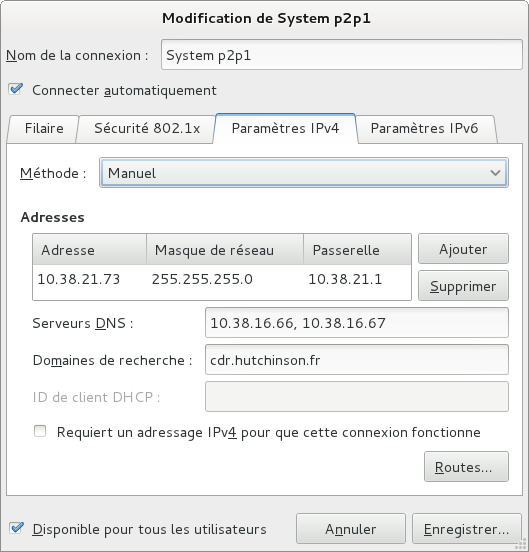
\includegraphics[scale=0.35]{img/Configuration_reseau.png}
%	\caption{Fenêtre de configuration du réseau}
%	\label{Fenêtre de configuration du réseau}
%\end{figure}

%Il est possible d'utiliser l'interface graphique pour modifier les différents paramètres, montrée sur la capture d'écran \ref{Fenêtre de configuration du réseau}, mais dans le cas de la machine virtuelle minimale cette fenêtre est indisponible.
Il est possible d'utiliser l'interface graphique pour modifier les différents paramètres, mais dans le cas de la machine virtuelle minimale cette fenêtre est indisponible.
Tous les réglages doivent donc se faire en ligne de commande ou dans des fichiers de configuration.
\\


Le fichier \lstinline{/etc/sysconfig/network-scripts/ifcfg-p2p1} contient toute la configuration de l'interface réseau utilisé par la machine virtuelle.
Il est mis à jour automatiquement à chaque changement d'options dans l'interface graphique.

Pour permettre la connexion au réseau et à internet, il suffira de modifier le fichier de cette manière :
\begin{lstlisting}
HWADDR=08:00:27:E7:B2:0E
ONBOOT=yes
IPADDR0=10.38.21.79
NETMASK=255.255.255.0
DNS1=10.38.16.66
DNS2=10.38.16.67
\\
\end{lstlisting}



%%%%%%%%%%%%%%%%%%%%%%%%%%%%%%%%%%%%%%%%%%%%%%%%%%%%%%%%%%%%%%%%%%%%%%%%%%%%%%%%%%%%%%%%%%%%%%%%%%%%

\subsubsection{Le service "network"}
\label{Le service "network"}

Un \textit{service} est un démon, c'est à dire un processus qui s'exécute en tâche de fond dans le système.
Ils sont démarrés par le processus de base, \textit{init} dont le PID 1, lors du démarrage du système.

\textit{network} est le service qui gère l'ensemble du réseau sur le système, tels que la carte réseau, la table de routage, \ldots
\\


Il existe plusieurs niveaux de démarrage sous Linux :
\begin{enumerate}
	\item 0 : Il produit l'extinction du système ;
	\item 1 : C'est le mode mono-utilisateur, utilisable uniquement en "root", pour la maintenance par exemple ;
	\item 2, 3 : Mode multi-utilisateur ;
	\item 5 : Mode multi-utilisateur, avec serveur graphique (X11) ;
	\item 6 : Il produit le redémarrage du système.
\end{enumerate}
Selon le niveaux utilisé, les différents services ne sont pas démarrés avec le système.

Par défaut, la machine virtuelle complète démarre en niveau 5 avec interface graphique et l'ensemble des services.
Par contre, la machine minimale, qui ne dispose pas d'interface graphique, démarre en niveau 3 et ne dispose pas du service réseau.
\\


Pour activer un service dans un niveau particulier, la technique simple et propre consiste à utiliser la commande \lstinline{chkconfig}.
En option, il faut préciser le niveau de démarrage, le service à modifier, puis son état de démarrage :
\begin{lstlisting}
chkconfig --level <niveau> <service> <on/off>
\end{lstlisting}

Pour activer le réseau de la machine minimale, la commande à utiliser est donc :
\begin{lstlisting}
chkconfig --level 3 network on
\end{lstlisting}
Une fois exécutée, le service sera automatiquement démarré lors des prochains démarrage du système. 
\\



%%%%%%%%%%%%%%%%%%%%%%%%%%%%%%%%%%%%%%%%%%%%%%%%%%%%%%%%%%%%%%%%%%%%%%%%%%%%%%%%%%%%%%%%%%%%%%%%%%%%

\subsubsection{La table de routage}

La table de routage est une structure de données définissant le cheminement des données dans un routeur ou un ordinateur en réseau.
Elle est géré dynamiquement par le système.

En effectuant les différentes configurations, j'ai remarqué que la table de routage n'était pas correcte, et que cela empêchait d'avoir accès au réseau.
\\


Tout d'abord, une ligne de la table perturbait le bon fonctionnement.
Tant qu'elle est présente, il sera impossible d'accéder au réseau.
La solution consiste à supprimer cette ligne à chaque démarrage du système.

Le fichier \lstinline{/etc/profile} est commun à tous les utilisateurs, et permet de configurer le Shell.
Les commandes présentes dans ce fichier seront exécutées lors du démarrage.
Pour effacer la ligne de la table de routage, il suffit donc d'y ajouter la commande :
\begin{lstlisting}
ip route delete 10.0.0.0/8 dev p2p1
\end{lstlisting}
~~\\


Ensuite, il manque certaines entrées qui permettent d'accéder à la passerelle et au proxy utilisé par l'entreprise.
Il est possible de les ajouter manuellement dans le fichier \lstinline{/etc/sysconfig/network-scripts/route-p2p1}, pour que le service (network) les ajoute à chaque démarrage.

Pour cela, on ajoutera les lignes suivantes :
\begin{lstlisting}
ADDRESS0=10.38.21.0
GATEWAY0=0.0.0.0
NETMASK0=255.255.255.0
ADDRESS1=0.0.0.0
GATEWAY1=10.38.21.1
NETMASK1=0.0.0.0
\end{lstlisting}
~~\\



%%%%%%%%%%%%%%%%%%%%%%%%%%%%%%%%%%%%%%%%%%%%%%%%%%%%%%%%%%%%%%%%%%%%%%%%%%%%%%%%%%%%%%%%%%%%%%%%%%%%

\subsubsection{Le proxy}

Un proxy est un intermédiaire entre différents réseaux informatiques.
Il peut s'agir d'un serveur ou d'un programme.
Cela permet de filtrer les données entrantes et sortantes, souvent par mesure de sécurité.
\\


Sous Linux les paramètres du (ou des) proxy sont situés dans des variables d'environnement :
\begin{itemize}
	\item http\_proxy ;
	\item https\_proxy ;
	\item ftp\_proxy.
\end{itemize}

Pour que ces variables d'environnement soient définies lors du démarrage du système, il est possible d'ajouter les lignes suivantes dans le fichier \lstinline{/etc/profile} ce qui les définira automatiquement :
\begin{lstlisting}
export http_proxy=http://10.38.22.2:8080/
export ftp_proxy=http://10.38.22.2:8080/
export https_proxy=http://10.38.22.2:8080/
\end{lstlisting}
~~\\


Pour le programme \textit{yum}, le proxy se configure dans son fichier de configuration \lstinline{/etc/yum.conf} en ajoutant les lignes suivantes :
\begin{lstlisting}
proxy=http://<adresse>:<port>
proxy_username=<identifiant>
proxy_password=<mot_de_passe>
\end{lstlisting}
Dans mon cas, le proxy ne demande aucun identifiant ni mot de passe, j'ai donc ajouter la ligne :
\begin{lstlisting}
proxy=http://10.38.22.2:8080
\end{lstlisting}
~~\\





%%%%%%%%%%%%%%%%%%%%%%%%%%%%%%%%%%%%%%%%%%%%%%%%%%%%%%%%%%%%%%%%%%%%%%%%%%%%%%%%%%%%%%%%%%%%%%%%%%%%
%%%%%%%%%%%%%%%%%%%%%%%%%%%%%%%%%%%%%%%%%%%%%%%%%%%%%%%%%%%%%%%%%%%%%%%%%%%%%%%%%%%%%%%%%%%%%%%%%%%%
%%%%%%%%%%%%%%%%%%%%%%%%%%%%%%%%%%%%%%%%%%%%%%%%%%%%%%%%%%%%%%%%%%%%%%%%%%%%%%%%%%%%%%%%%%%%%%%%%%%%
%%%%%%%%%%%%%%%%%%%%%%%%%%%%%%%%%%%%%%%%%%%%%%%%%%%%%%%%%%%%%%%%%%%%%%%%%%%%%%%%%%%%%%%%%%%%%%%%%%%%
%%%%%%%%%%%%%%%%%%%%%%%%%%%%%%%%%%%%%%%%%%%%%%%%%%%%%%%%%%%%%%%%%%%%%%%%%%%%%%%%%%%%%%%%%%%%%%%%%%%%

\section{Installation d'un outil}

Dans cette partie, il s'agit de l'installation de MBDyn.
Tous les outils suivront cette procédure sauf pour l'étape de compilation qui sera précisée.
\\


Dans le cas présent, on notera :
\begin{itemize}
	\item \lstinline{/dev/sdb} : le fichier représentant le disque dans la machine virtuelle ;
	\item \lstinline{3f01e3c5-0ac1-4391-99fb-13be6595391b} : l'UUID du disque, qui est identique à celui de VirtualBox ;
	\item \lstinline{/opt/mbdyn} : le répertoire de montage du disque ;
	\item \lstinline{~/mbdyn-1.4.3} : le répertoire contenance la source de l'outil à installer.
\\
\end{itemize}


On se place préalablement en mode \textit{super-utilisateur} pour pouvoir exécuter les commandes administrateur et accéder aux répertoires protégés :
\begin{lstlisting}[language = sh]
$ su
\end{lstlisting}

La première étape consiste à formater le disque virtuel dans un format reconnu par Linux (\textit{ext2}) :
\begin{lstlisting}[language = sh]
# mke2fs -F /dev/sdb
\end{lstlisting}

On change l'UUID du disque, pour avoir le même UUID que VirtualBox :
\begin{lstlisting}[language = sh]
# tune2fs -U 3f01e3c5-0ac1-4391-99fb-13be6595391b /dev/sdb
\end{lstlisting}

On crée le répertoire de montage s'il n'existe pas, puis on monte le disque :
\begin{lstlisting}[language = sh]
# mkdir /opt/mbdyn
# mount -U 3f01e3c5-0ac1-4391-99fb-13be6595391b /opt/mbdyn
\end{lstlisting}

Ensuite on se place dans le répertoire source de l'outil, avant la compilation et l'installation standard.
C'est cette étape qui peut différer selon l'outil.
\begin{lstlisting}[language = sh]
$ cd ~/mbdyn-1.4.3
$ ./configure --prefix=/opt/mbdyn --disable-shared --enable-static
$ make
# make install
\end{lstlisting}

L'outil est ainsi installé dans le répertoire monté, c'est à dire dans le disque virtuel.
On peut démonter le disque avant de le débrancher de la machine virtuelle, en utilisant une des deux commandes :
\begin{lstlisting}[language = sh]
# umount /opt/mbdyn
# umount /dev/sdb
\end{lstlisting}
~~\\





%%%%%%%%%%%%%%%%%%%%%%%%%%%%%%%%%%%%%%%%%%%%%%%%%%%%%%%%%%%%%%%%%%%%%%%%%%%%%%%%%%%%%%%%%%%%%%%%%%%%
%%%%%%%%%%%%%%%%%%%%%%%%%%%%%%%%%%%%%%%%%%%%%%%%%%%%%%%%%%%%%%%%%%%%%%%%%%%%%%%%%%%%%%%%%%%%%%%%%%%%
%%%%%%%%%%%%%%%%%%%%%%%%%%%%%%%%%%%%%%%%%%%%%%%%%%%%%%%%%%%%%%%%%%%%%%%%%%%%%%%%%%%%%%%%%%%%%%%%%%%%
%%%%%%%%%%%%%%%%%%%%%%%%%%%%%%%%%%%%%%%%%%%%%%%%%%%%%%%%%%%%%%%%%%%%%%%%%%%%%%%%%%%%%%%%%%%%%%%%%%%%
%%%%%%%%%%%%%%%%%%%%%%%%%%%%%%%%%%%%%%%%%%%%%%%%%%%%%%%%%%%%%%%%%%%%%%%%%%%%%%%%%%%%%%%%%%%%%%%%%%%%

\section{Scripts SHELL}

Ce script permet d'installer l'ensemble des bibliothèques dynamiques manquantes dont dépend un exécutable, en téléchargeant les paquets nécessaires.
\\


\begin{landscape}
\begin{lstlisting}[language = sh]
#!/bin/bash

# Argument 1 : chemin de l'executable
EXE="$1"

# Tests sur l'executable d'entree
if [ ! -e "$EXE" ]
then
    echo "cible inexistante"
    exit
elif [ `file "$EXE" | grep 'executable' | wc -l` -eq 0 ]
then
    echo "cible non executable"
    exit
elif [ `file "$EXE" | grep 'dynamically linked' | wc -l` -eq 0 ]
then
    echo "executable non dynamique"
    exit
fi

# Tuer les processus utilisant YUM
kill -9 `ps aux | grep yum | cut -d " " -f 7` 2>/dev/null

# Parcours des bibliotheques manquantes
for LIB_LibNomExt in `ldd $EXE | grep 'not found' | sed "s/ => .*//"`
do
    echo -n "$LIB_LibNomExt : "
    
    # Installee en meme temps qu'une dependance precedente
    if [ `ldd "$EXE" | grep "$LIB_LibNomExt => not found" | wc -l` -eq 0 ]
    then
        echo "installee"
        continue
    fi
    
    LIB_Nom=`echo "$LIB_LibNomExt" | sed "s/\.so\.[0-9]$//" | sed "s/^lib//"`
    
    # La bibliotheque est directement dans le depot
    if [ `yum search "$LIB_Nom" 2>/dev/null | grep "^$LIB_Nom.x86_64 : " | wc -l` -ne 0 ]
    then
        Pack="$LIB_Nom"
    else
        # Rechercher la bibliotheque dans les autres paquets
        Ligne2=`yum provides "$LIB_LibNomExt" | sed -n '2p'`
        if [ `echo $Ligne2 | grep '^No Matches found$' | wc -l` -ne 0 ]
        then
            echo "introuvable"
            continue
        else
            PACK_Nom=`echo "$Ligne2" | sed "s/ : .*$//" | sed "s/\.[a-z0-9_]*$//" \
            						 | sed "s/-[a-z0-9.]*$//" | sed "s/-[0-9.]*$//"`
            # Verifier que le paquet est dans le depot
            if [ `yum search "$PACK_Nom" | grep "^$PACK_Nom.x86_64 : " | wc -l` -eq 0 ]
            then
                echo "introuvable"
                continue
            else
                Pack="$PACK_Nom"
            fi
        fi
    fi
    
    # Installation du paquet
    sudo yum install -y "$Pack" >/dev/null 2>&1
    
    # Verification de l'installation
    if [ `ldd "$EXE" | grep "$LIB_LibNomExt => not found" | wc -l` -ne 0 ]
    then
        echo "echec de l'installation"
    else
        echo "installee"
    fi
done

# Verifications
if [ `ldd "$EXE" | grep 'not found' | wc -l` -ne 0 ]
then
    echo "Dependances manquantes"
else
    echo "Dependances installees"
fi
\end{lstlisting}
\end{landscape}





%%%%%%%%%%%%%%%%%%%%%%%%%%%%%%%%%%%%%%%%%%%%%%%%%%%%%%%%%%%%%%%%%%%%%%%%%%%%%%%%%%%%%%%%%%%%%%%%%%%%
%%%%%%%%%%%%%%%%%%%%%%%%%%%%%%%%%%%%%%%%%%%%%%%%%%%%%%%%%%%%%%%%%%%%%%%%%%%%%%%%%%%%%%%%%%%%%%%%%%%%
%%%%%%%%%%%%%%%%%%%%%%%%%%%%%%%%%%%%%%%%%%%%%%%%%%%%%%%%%%%%%%%%%%%%%%%%%%%%%%%%%%%%%%%%%%%%%%%%%%%%
%%%%%%%%%%%%%%%%%%%%%%%%%%%%%%%%%%%%%%%%%%%%%%%%%%%%%%%%%%%%%%%%%%%%%%%%%%%%%%%%%%%%%%%%%%%%%%%%%%%%
%%%%%%%%%%%%%%%%%%%%%%%%%%%%%%%%%%%%%%%%%%%%%%%%%%%%%%%%%%%%%%%%%%%%%%%%%%%%%%%%%%%%%%%%%%%%%%%%%%%%

\section{Résultats des tests d'échange}

Ces graphiques résultent des tests d'échange développés dans la partie \ref{Comparaison}.
\\


\begin{figure}[!h]
	\center
	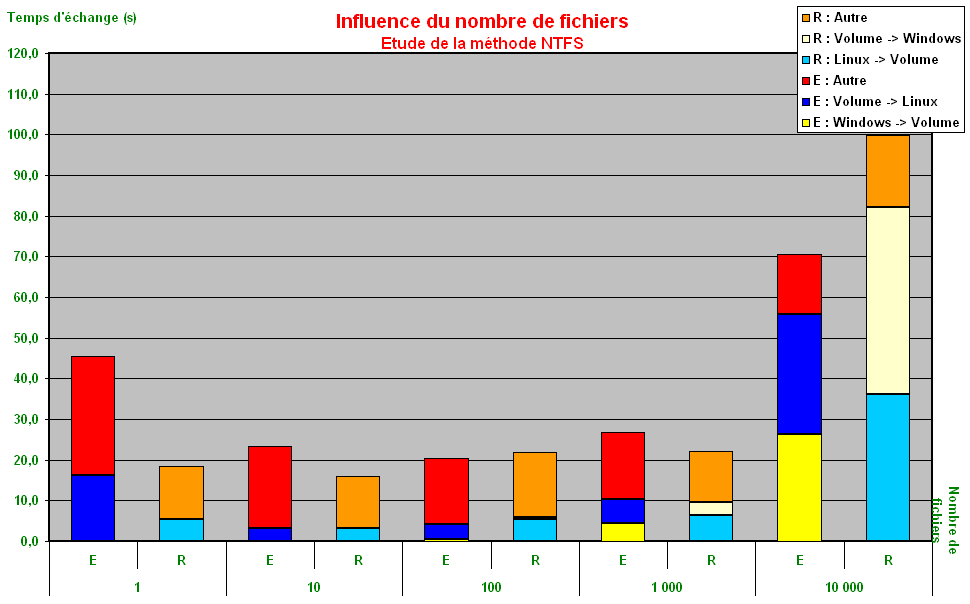
\includegraphics[scale=0.4]{img/tests/nombre_NTFS.png}
	\caption{Temps d'échange en fonction du nombre de fichiers}
	Méthode du disque virtuel
\end{figure}

\begin{figure}[!h]
	\center
	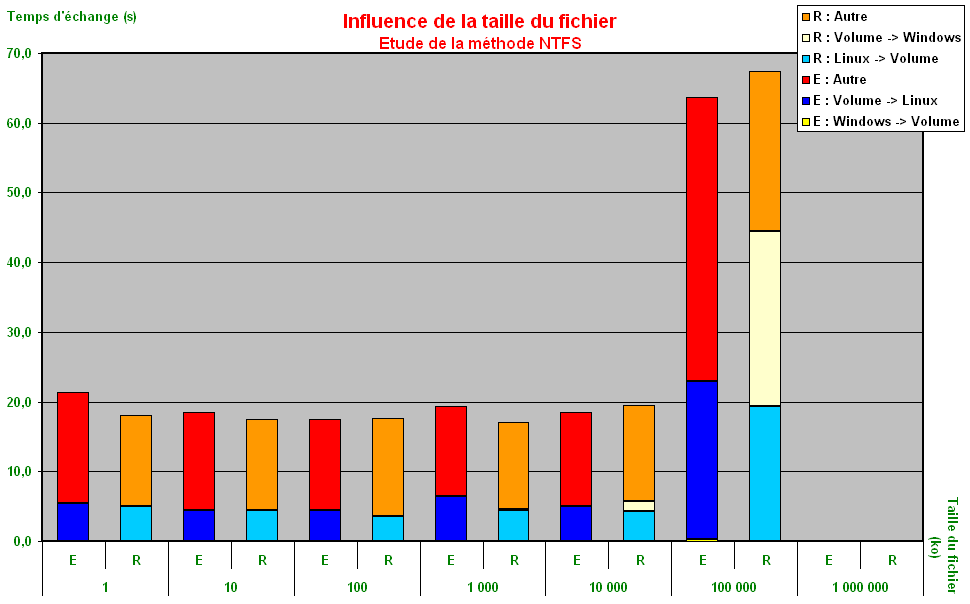
\includegraphics[scale=0.4]{img/tests/taille_NTFS.png}
	\caption{Temps d'échange fonction de la taille du fichier}
	Méthode du disque virtuel
\end{figure}

\begin{figure}[!h]
	\center
	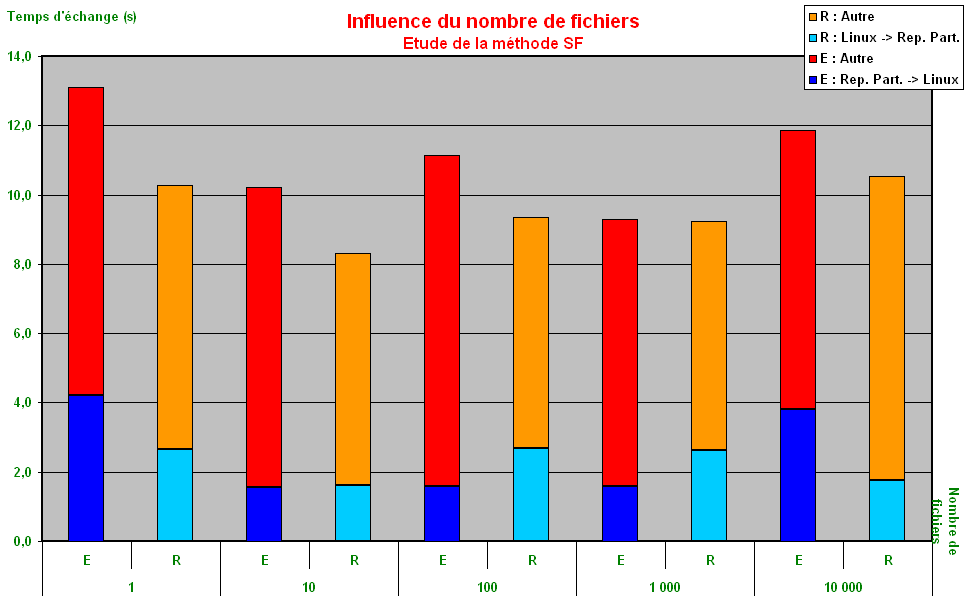
\includegraphics[scale=0.4]{img/tests/nombre_SF.png}
	\caption{Temps d'échange en fonction du nombre de fichiers}
	Méthode du répertoire partagé
\end{figure}

\begin{figure}[!h]
	\center
	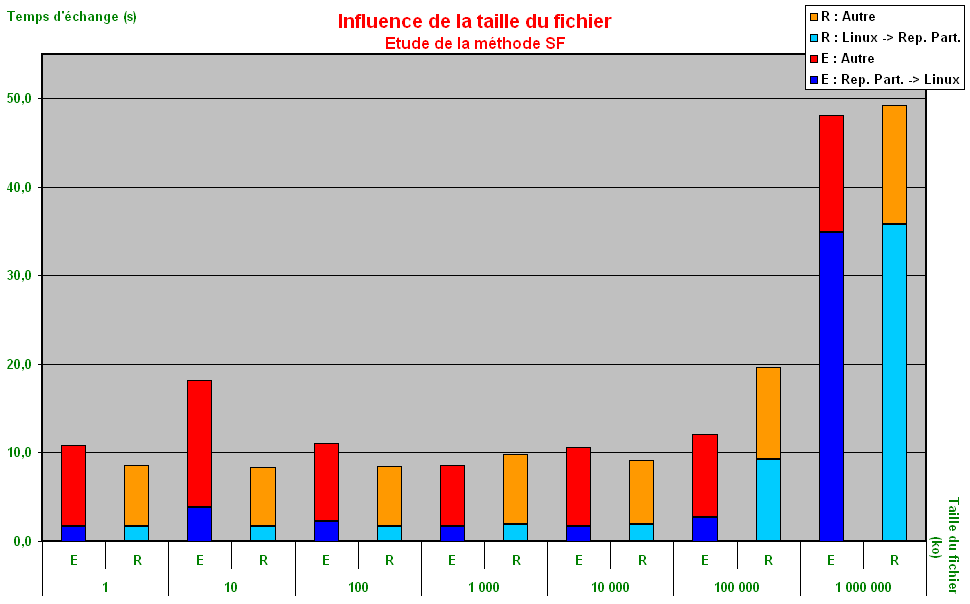
\includegraphics[scale=0.4]{img/tests/taille_SF.png}
	\caption{Temps d'échange fonction de la taille du fichier}
	Méthode du répertoire partagé
\end{figure}